\documentclass[UTF8,11pt,a4paper,oneside,fontset=none]{ctexart}

\usepackage[a4paper,top=1.75cm,bottom=1.75cm,left=1.85cm,right=1.85cm,headheight=15pt]{geometry}
\usepackage{fontspec}
\usepackage{amsmath,amssymb,mathtools,bm}
\usepackage{unicode-math}
\usepackage{booktabs,tabularx,array,multirow}
\usepackage[table]{xcolor}
\usepackage{graphicx,float}
\usepackage{siunitx}
\usepackage{enumitem}
\usepackage{fancyhdr}
\usepackage{caption}
\usepackage{hyperref}
\usepackage[most]{tcolorbox}

\setmainfont{Times New Roman}
\setsansfont{Arial}
\setmonofont{Consolas}
\setmathfont{Cambria Math}
\setCJKmainfont[BoldFont=SimHei,ItalicFont=KaiTi]{SimSun}
\setCJKsansfont[BoldFont={Microsoft YaHei Bold}]{Microsoft YaHei}
\setCJKmonofont{FangSong}

\definecolor{DeepBlue}{HTML}{17324D}
\definecolor{PandaTeal}{HTML}{0B7A75}
\definecolor{WarmGold}{HTML}{C58A19}
\definecolor{Coral}{HTML}{C95F4A}
\definecolor{SoftBlue}{HTML}{EEF5F8}
\definecolor{SoftTeal}{HTML}{ECF7F5}
\definecolor{SoftGold}{HTML}{FFF7E7}
\definecolor{SoftRed}{HTML}{FFF0F0}
\definecolor{MidGray}{HTML}{667085}
\definecolor{LineGray}{HTML}{D5DEE5}

\hypersetup{colorlinks=true,linkcolor=DeepBlue,urlcolor=PandaTeal,
  pdfauthor={范子恒},pdftitle={PandaX-4T run10972 原始数据报告}}
\ctexset{
  section={format=\Large\bfseries\color{DeepBlue},number=\arabic{section},beforeskip=0pt,afterskip=0.8em},
  subsection={format=\large\bfseries\color{PandaTeal}}
}

\pagestyle{fancy}
\fancyhf{}
\fancyhead[L]{\small\color{DeepBlue}PandaX-4T run10972}
\fancyhead[R]{\small\color{MidGray}原始数据报告}
\fancyfoot[C]{\small\color{MidGray}\thepage}
\renewcommand{\headrulewidth}{0.4pt}
\renewcommand{\footrulewidth}{0pt}

\captionsetup{font=small,labelfont=bf,labelsep=quad}
\graphicspath{{figures/}}
\setlength{\parindent}{2em}
\setlength{\parskip}{0.18em}
\setlist[itemize]{leftmargin=1.6em,itemsep=0.25em,topsep=0.25em,parsep=0pt}
\setlist[enumerate]{leftmargin=1.8em,itemsep=0.28em,topsep=0.25em,parsep=0pt}
\renewcommand{\arraystretch}{1.18}
\sisetup{group-separator={,},group-minimum-digits=4,range-phrase={--},range-units=single}

\newcolumntype{Y}{>{\raggedright\arraybackslash}X}
\newcolumntype{C}[1]{>{\centering\arraybackslash}p{#1}}
\newcolumntype{R}[1]{>{\raggedleft\arraybackslash}p{#1}}
\newtcolorbox{infobox}[1][]{enhanced,breakable,colback=SoftBlue,colframe=DeepBlue,
  boxrule=0.7pt,arc=1.7mm,left=1.4mm,right=1.4mm,top=1mm,bottom=1mm,#1}
\newtcolorbox{scopebox}[1][]{enhanced,breakable,colback=SoftRed,colframe=Coral,
  boxrule=0.75pt,arc=1.7mm,title={数据边界},fonttitle=\bfseries,
  left=1.4mm,right=1.4mm,top=1mm,bottom=1mm,#1}
\newtcolorbox{notebox}[1][]{enhanced,breakable,colback=SoftGold,colframe=WarmGold,
  boxrule=0.75pt,arc=1.7mm,title={解释说明},fonttitle=\bfseries,
  left=1.4mm,right=1.4mm,top=1mm,bottom=1mm,#1}
\newtcolorbox{conclusionbox}[1][]{enhanced,breakable,colback=SoftTeal,colframe=PandaTeal,
  boxrule=0.85pt,arc=1.7mm,title={本页结论},fonttitle=\bfseries,
  left=1.4mm,right=1.4mm,top=1mm,bottom=1mm,#1}

\newcommand{\Sone}{\mathrm{S1}}
\newcommand{\StwoB}{\mathrm{S2}_{\mathrm B}}
\newcommand{\SoneLY}{\mathrm{S1}}
\newcommand{\StwoLY}{\mathrm{S2B}}

\begin{document}

% 第 1 页：封面
\thispagestyle{empty}
\vspace*{1.0cm}
\noindent{\color{PandaTeal}\rule{\textwidth}{3.5pt}}
\vspace{1.05cm}

{\sffamily\bfseries\fontsize{25pt}{32pt}\selectfont\color{DeepBlue}
PandaX-4T run10972\par 原始数据报告\par}
\vspace{0.35cm}
{\sffamily\bfseries\fontsize{16pt}{22pt}\selectfont\color{PandaTeal}
上游标量输入数据的结构、质量与基础分布\par}

\vspace{0.85cm}
\begin{tcolorbox}[colback=SoftBlue,colframe=DeepBlue,boxrule=0.9pt,arc=2mm,
  left=3mm,right=3mm,top=2.5mm,bottom=2.5mm]
\centering
{\sffamily\bfseries\large 报告目的}\par\vspace{1mm}
说明当前输入数据是什么、五个物理观测量是否完整，\par
并记录信号相关性、漂移时间分布和空间覆盖。\par
本报告只描述输入数据，不评价后续重建方法的性能。
\end{tcolorbox}

\vspace{0.72cm}
\begin{center}
\begin{tabular}{C{4.7cm} C{4.7cm} C{4.7cm}}
\begin{tcolorbox}[width=4.45cm,colback=white,colframe=LineGray,arc=1.5mm,halign=center]
{\sffamily\bfseries\fontsize{22pt}{24pt}\selectfont\color{DeepBlue}4500}\par\small 筛选后事件
\end{tcolorbox}
&
\begin{tcolorbox}[width=4.45cm,colback=white,colframe=LineGray,arc=1.5mm,halign=center]
{\sffamily\bfseries\fontsize{22pt}{24pt}\selectfont\color{PandaTeal}188}\par\small 输入字段
\end{tcolorbox}
&
\begin{tcolorbox}[width=4.45cm,colback=white,colframe=LineGray,arc=1.5mm,halign=center]
{\sffamily\bfseries\fontsize{22pt}{24pt}\selectfont\color{WarmGold}5}\par\small 物理观测量
\end{tcolorbox}
\end{tabular}
\end{center}

\vspace{0.38cm}
\begin{scopebox}[title={“原始数据”的准确含义}]
这里的“原始数据”是本项目直接收到并开始分析的上游标量表，而不是未经处理的探测器波形。数据名称中的 \texttt{finalSS} 和 \texttt{Egt2MeV} 暗示它很可能已经经过单散射与能量阈值等上游选择。
\end{scopebox}

\vfill
\begin{tabularx}{\textwidth}{@{}Y R{5.2cm}@{}}
\textbf{报告人：}范子恒 & \textbf{数据：}run10972\\
\textbf{用途：}原始数据说明 & \textbf{版本：}基础变量精简版
\end{tabularx}
\vspace{0.30cm}
\noindent{\color{PandaTeal}\rule{\textwidth}{1.3pt}}
\clearpage

% 第 2 页：数据来源与边界
\section{数据来源与使用边界}

当前输入为一张制表符分隔的事件级标量表。每一行表示一个已经被上游流程保留的事件，每一列表示一个标识量、信号量、位置量、形状量、计数、选择标志或派生量。本项目不覆盖原表，也不把全部 188 个字段直接送入模型。

\vspace{0.35em}
\begin{minipage}[t]{0.55\textwidth}
\rowcolors{2}{SoftBlue}{white}
\begin{tabularx}{\linewidth}{@{}Y R{3.15cm}@{}}
\toprule
\rowcolor{DeepBlue!11}\textbf{审计项目} & \textbf{结果}\\
\midrule
运行号 & 10972\\
事件数（行数） & \num{4500}\\
字段数（列数） & 188\\
实际读取列 & 7\\
物理观测量 & 5\\
五个观测量有限值 & \num{4500}/\num{4500}\\
S1、S2 信号为正 & \num{4500}/\num{4500}\\
漂移时间范围 & \SIrange{10.1}{842.3}{\micro\second}\\
漂移时间中位数 & \SI{417.8}{\micro\second}\\
半径中位数 & \SI{359.1}{\milli\metre}\\
\bottomrule
\end{tabularx}
\end{minipage}\hfill
\begin{minipage}[t]{0.41\textwidth}
\begin{infobox}[title={分析入口},fonttitle=\bfseries]
读取七列：
\begin{itemize}
  \item 来源元数据：\texttt{runNumber}、\texttt{eventNumber}；
  \item 信号：\texttt{qS1\_max}、\texttt{qS2B\_max}；
  \item 位置与时间：\texttt{xS2T\_max}、\texttt{yS2T\_max}、\texttt{dt}。
\end{itemize}
其中只有后五列是物理观测量。
\end{infobox}

\vspace{0.35em}
\begin{notebox}[title={事件对齐方式}]
读取后立即按原 TXT 行顺序生成
\[
  \texttt{sourceRow}=0,1,\ldots,4499.
\]
它只用于把图表和结果精确对应回输入行，不具有物理含义，不进入模型、校正公式或参数选择。
\end{notebox}
\end{minipage}

\vspace{0.55em}
\begin{scopebox}
4500 表示当前表中已经保留下来的事件数，不是 DAQ 的总触发数，也不能用于计算原始采集效率。188 表示表头中的全部字段数，不表示这些字段都已被确认可用。有关能量阈值、单散射效率或完整探测器接受率的结论，都需要额外的上游处理说明。
\end{scopebox}

\begin{conclusionbox}
本报告研究的是一个固定的、已经筛选过的 4500 事件样本。后续分析只使用明确的基础观测量，不把来源元数据或对齐索引解释为探测器响应。
\end{conclusionbox}
\clearpage

% 第 3 页：变量说明
\section{读取列与基本变量}

为了与后续公式保持一致，本报告将原表中的信号和位置列使用简短别名表示。读取列、角色和使用方式如下。

\small
\rowcolors{2}{SoftBlue}{white}
\begin{tabularx}{\textwidth}{@{}C{3.0cm} C{2.25cm} C{2.2cm} Y@{}}
\toprule
\rowcolor{DeepBlue!11}\textbf{读取列} & \textbf{本文记号} & \textbf{单位/类型} & \textbf{作用}\\
\midrule
\texttt{runNumber} & --- & 整数元数据 & 确认当前样本属于 run10972，不进入物理模型\\
\texttt{eventNumber} & --- & 整数元数据 & 保留上游事件标签，不作为唯一对齐键，不进入物理模型\\
\texttt{qS1\_max} & \(\SoneLY\) & p.e. & 主 S1 候选的总光电子量\\
\texttt{qS2B\_max} & \(\StwoLY\) & p.e. & 底部阵列主 S2 候选的光电子量\\
\texttt{dt} & \(t_{\mathrm d}\) & 原字段/1000 & S2 与 S1 的时间间隔，换算为漂移时间\\
\texttt{xS2T\_max} & \(x\) & mm & 主 S2 顶部位置重建的横向坐标\\
\texttt{yS2T\_max} & \(y\) & mm & 与 \(x\) 一起描述横向位置\\
\bottomrule
\end{tabularx}
\normalsize

\vspace{0.55em}
五个物理观测量构成事件向量
\begin{equation}
  \symbf{x}_i=
  \bigl(\SoneLY_i,\StwoLY_i,t_{\mathrm d,i},x_i,y_i\bigr),
  \qquad i=0,1,\ldots,4499.
\end{equation}
漂移时间与半径定义为
\begin{align}
  t_{\mathrm d} &= \frac{\texttt{dt}}{1000}
  \quad [\mu\mathrm{s}],\\
  r &= \sqrt{x^2+y^2}
  \quad [\mathrm{mm}].
\end{align}
半径 \(r\) 是由 \(x,y\) 立即计算的派生坐标，不是额外读取的输入列。

\begin{notebox}[title={S1 与 S2 表示什么？}]
粒子在液氙中沉积能量后，能量会在闪烁光和电离电子之间分配。S1 对应液相中的瞬发闪烁；漂移电子到达液面并被抽取到气相后产生电致发光，形成 S2。本数据使用底部阵列的 S2 光电子量作为第二个信号通道。
\end{notebox}

\begin{scopebox}
当前列名和单位来自已有变量说明与数据数值尺度。没有已知源线、增益参数 \(g_1,g_2\) 和完整选择条件时，不能由这些基础变量直接宣布绝对 MeV 能量或最终物理分辨率。
\end{scopebox}

\begin{conclusionbox}
真正进入物理描述的只有 S1、S2、漂移时间和两个横向坐标。\texttt{sourceRow} 只是可复现的对齐工具，与能量和位置无关。
\end{conclusionbox}
\clearpage

% 第 4 页：S1--S2
\section{S1--S2 联合分布}

\begin{figure}[H]
  \centering
  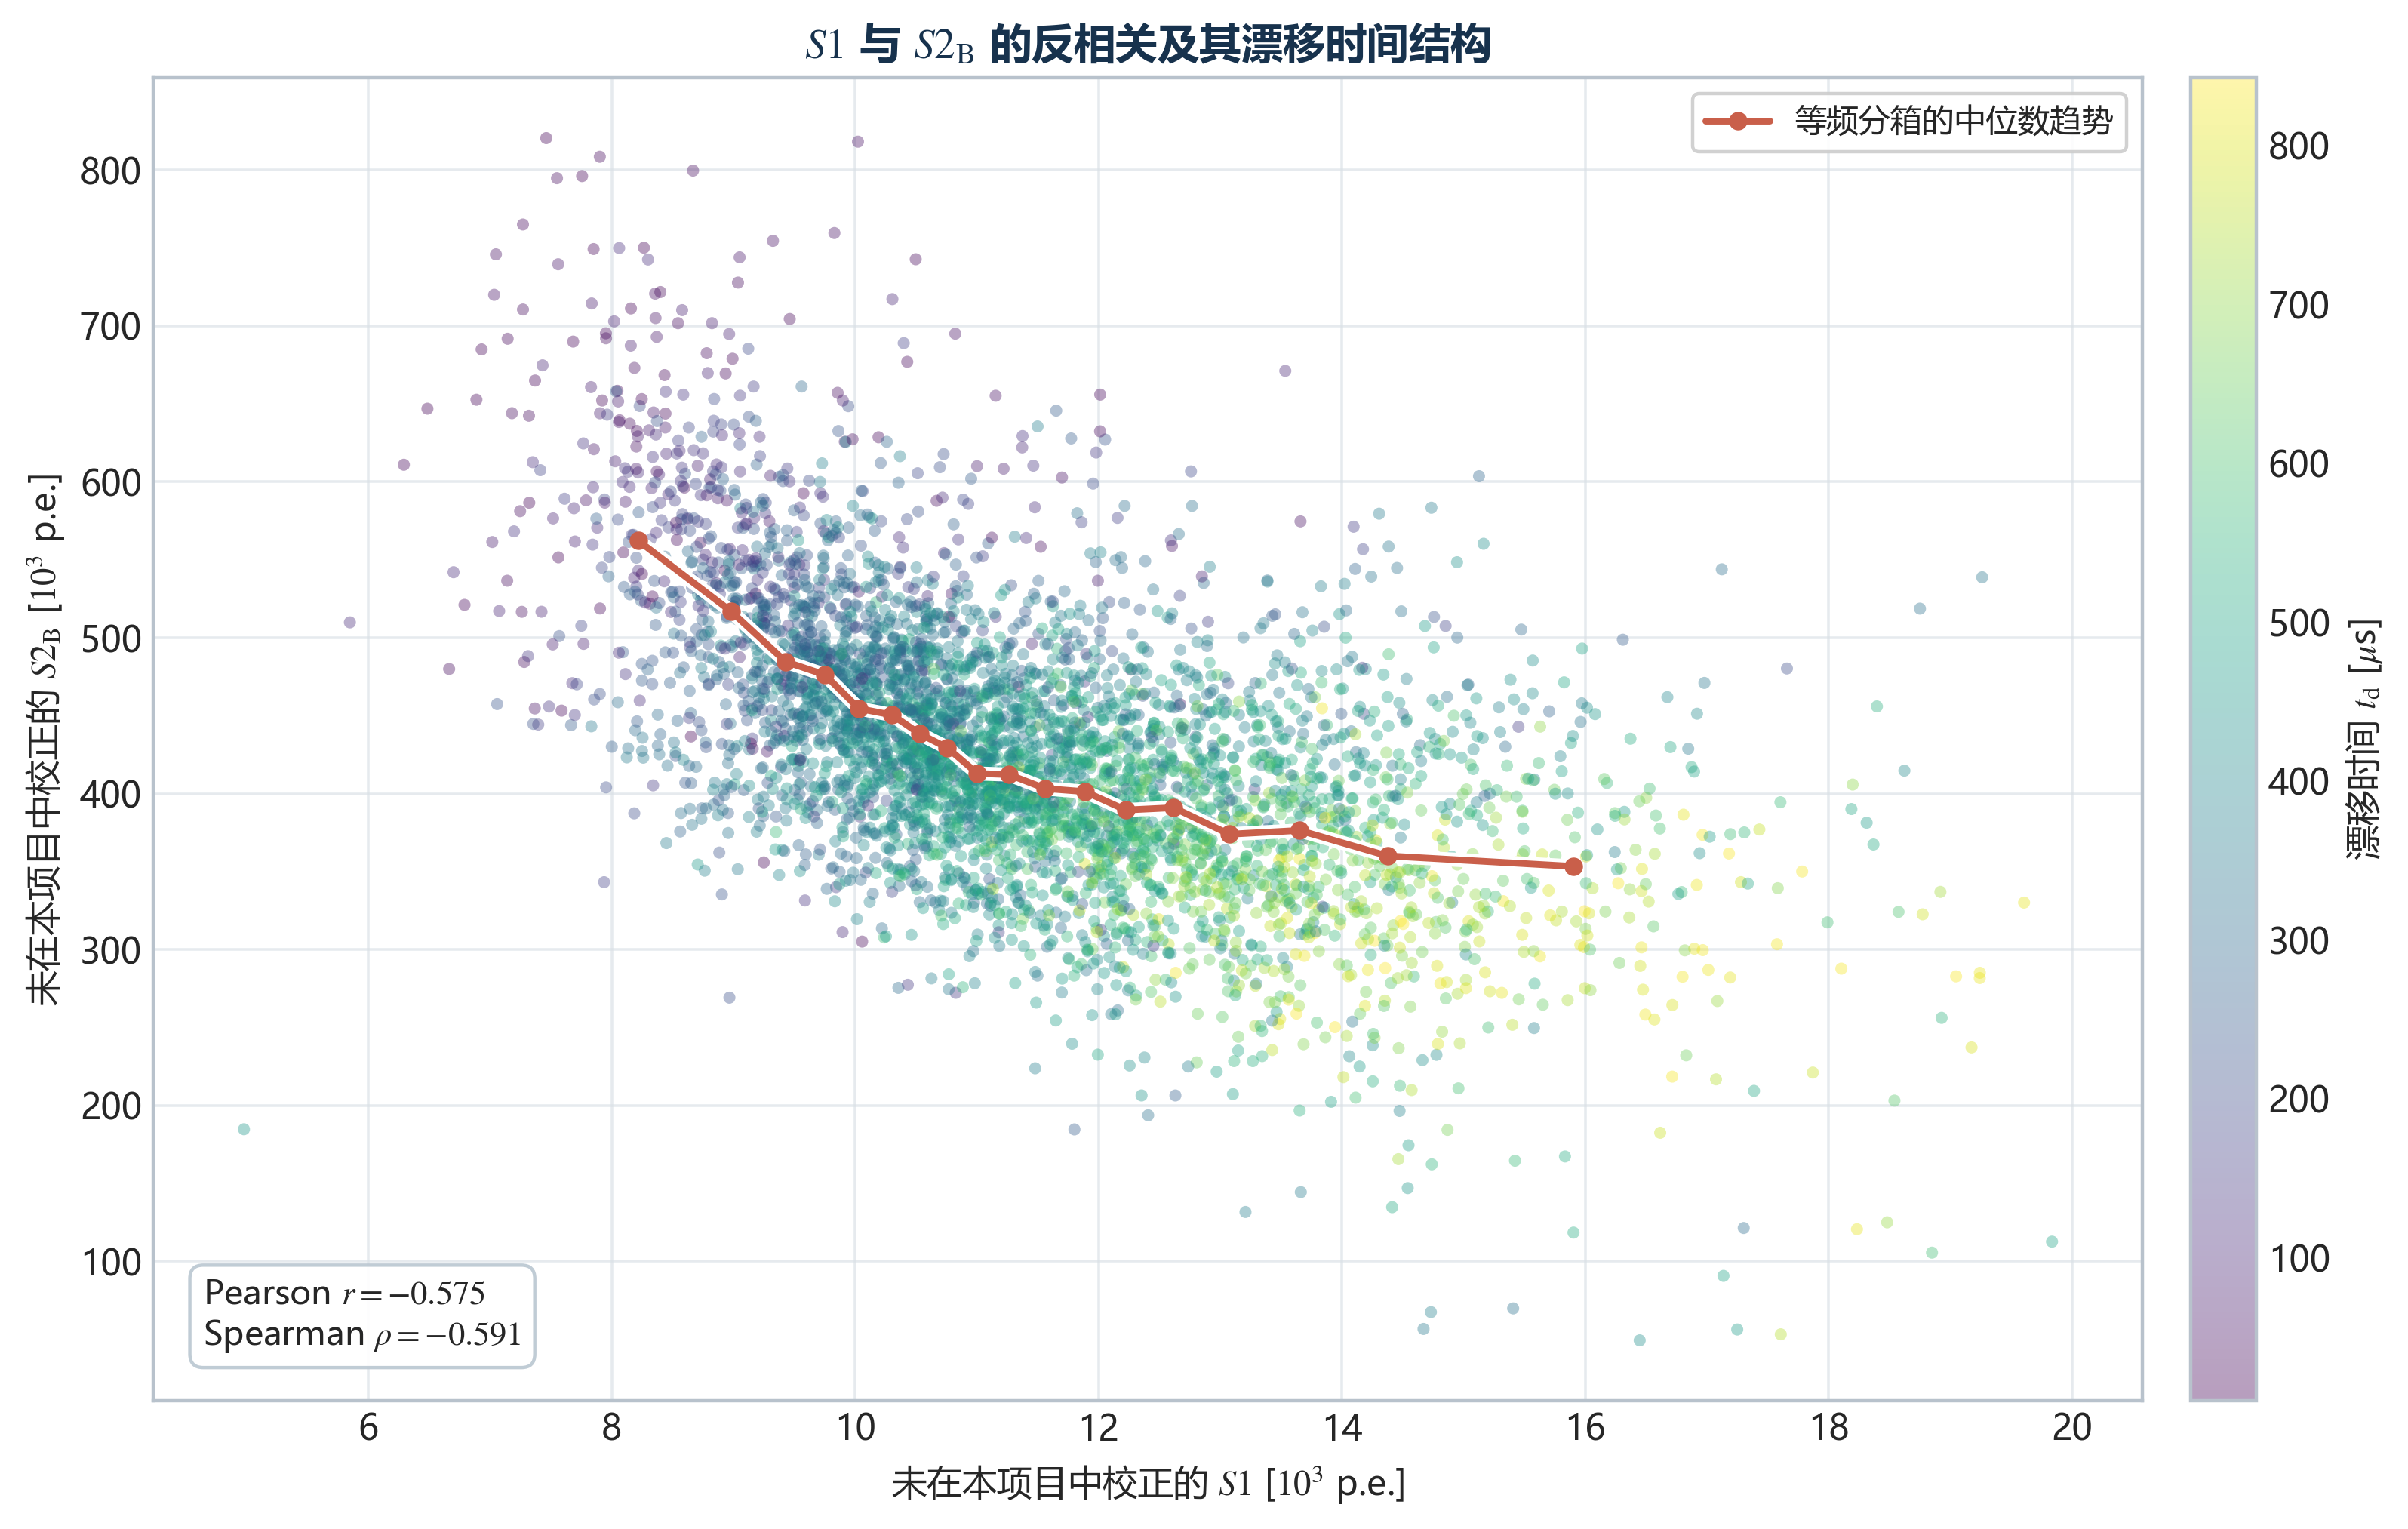
\includegraphics[width=0.93\textwidth]{02_s1_s2_anticorrelation_cn.png}
  \caption{每个点表示一个筛选后事件；横轴为输入 S1，纵轴为输入底部 S2，颜色表示漂移时间。红色折线连接 S1 等频分箱中的中位数点，只用于显示总体趋势。}
\end{figure}

图中的事件云整体由左上向右下倾斜：S1 较大的事件往往具有较小的 S2，反之亦然。这种反相关与液氙中光信号和电离信号之间的能量分配相符，也是把两个通道联合用于能量估计的直接数据依据。

\begin{infobox}[title={怎样读颜色？},fonttitle=\bfseries]
颜色编码的是漂移时间，而不是事件好坏或能量大小。不同颜色在点云中的分布并不完全相同，说明 S1--S2 联合响应还可能受到纵向位置的影响。
\end{infobox}

\begin{scopebox}
红色折线不是能量拟合曲线，也不是校正函数。仅凭点云斜率不能唯一确定 \(g_1\)、\(g_2\)、源能量或能量分辨率；点云还同时混合了上游选择、空间响应和真实物理谱形。
\end{scopebox}

\begin{conclusionbox}
S1 与 S2 存在清楚的反相关，说明两条通道包含互补信息；同时，漂移时间颜色结构提示后续处理必须检查位置依赖。
\end{conclusionbox}
\clearpage

% 第 5 页：空间覆盖
\section{漂移时间与空间覆盖}

\begin{figure}[H]
  \centering
  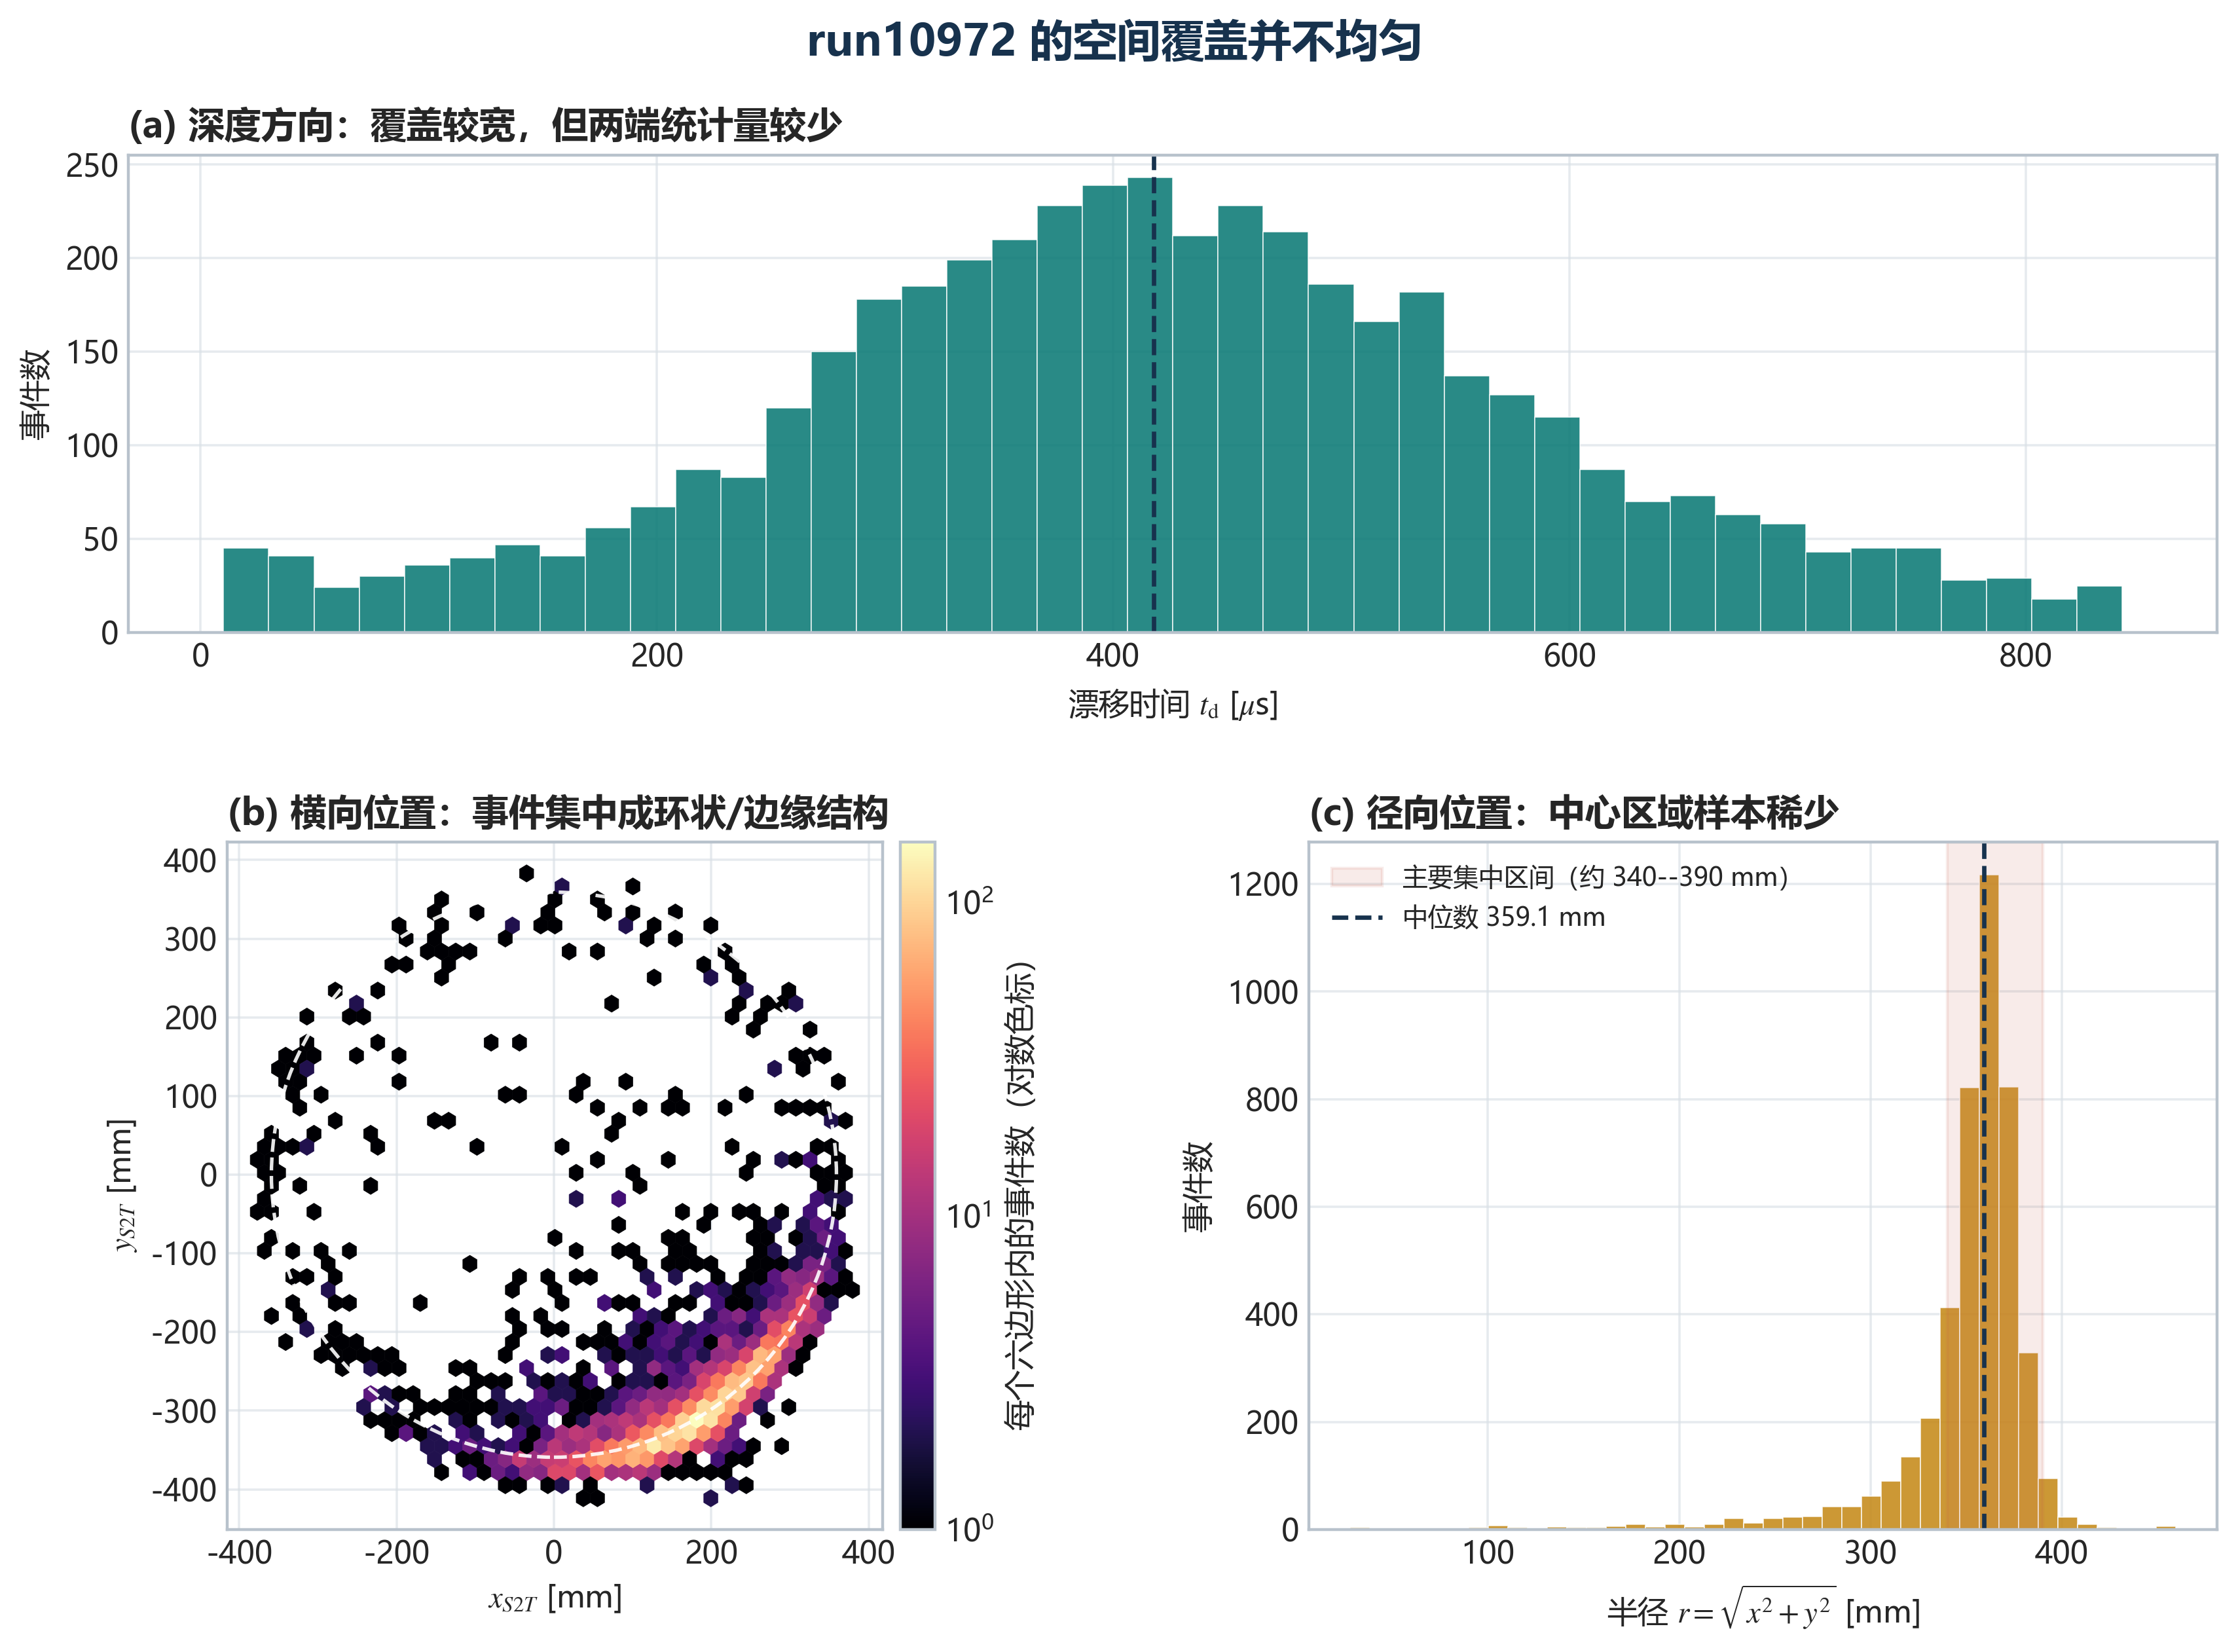
\includegraphics[width=0.92\textwidth]{03_spatial_coverage_cn.png}
  \caption{漂移时间、横向位置与半径的描述性分布。颜色密度只表示当前筛选后事件的集中程度。}
\end{figure}

漂移时间覆盖了较宽区间，但两端事件较少；横向位置并非均匀填满圆形区域，而是在外半径和部分方位明显集中。半径分布的中位数约为 \SI{359.1}{\milli\metre}，中心区域样本相对稀少。

\begin{notebox}[title={为什么这很重要？}]
若探测器响应随深度或半径变化，而样本又在某些位置过度集中，那么全局峰宽会同时受到“响应不均匀”和“样本位置分布”的影响。后续修正必须只在训练事件上学习响应，并在未参与学习的事件上评价。
\end{notebox}

\begin{scopebox}
当前分布不能被解释为探测器的几何接受率或源的真实空间分布，因为样本已经经过上游选择，而且缺少完整效率信息。
\end{scopebox}

\begin{conclusionbox}
样本在纵向和横向都不均匀；位置依赖是需要检验的主要系统效应，也限制了当前结果向其他 run 或其他源位置外推。
\end{conclusionbox}
\clearpage

% 第 6 页：条件趋势与数据结论
\section{基础条件趋势与数据结论}

\begin{figure}[H]
  \centering
  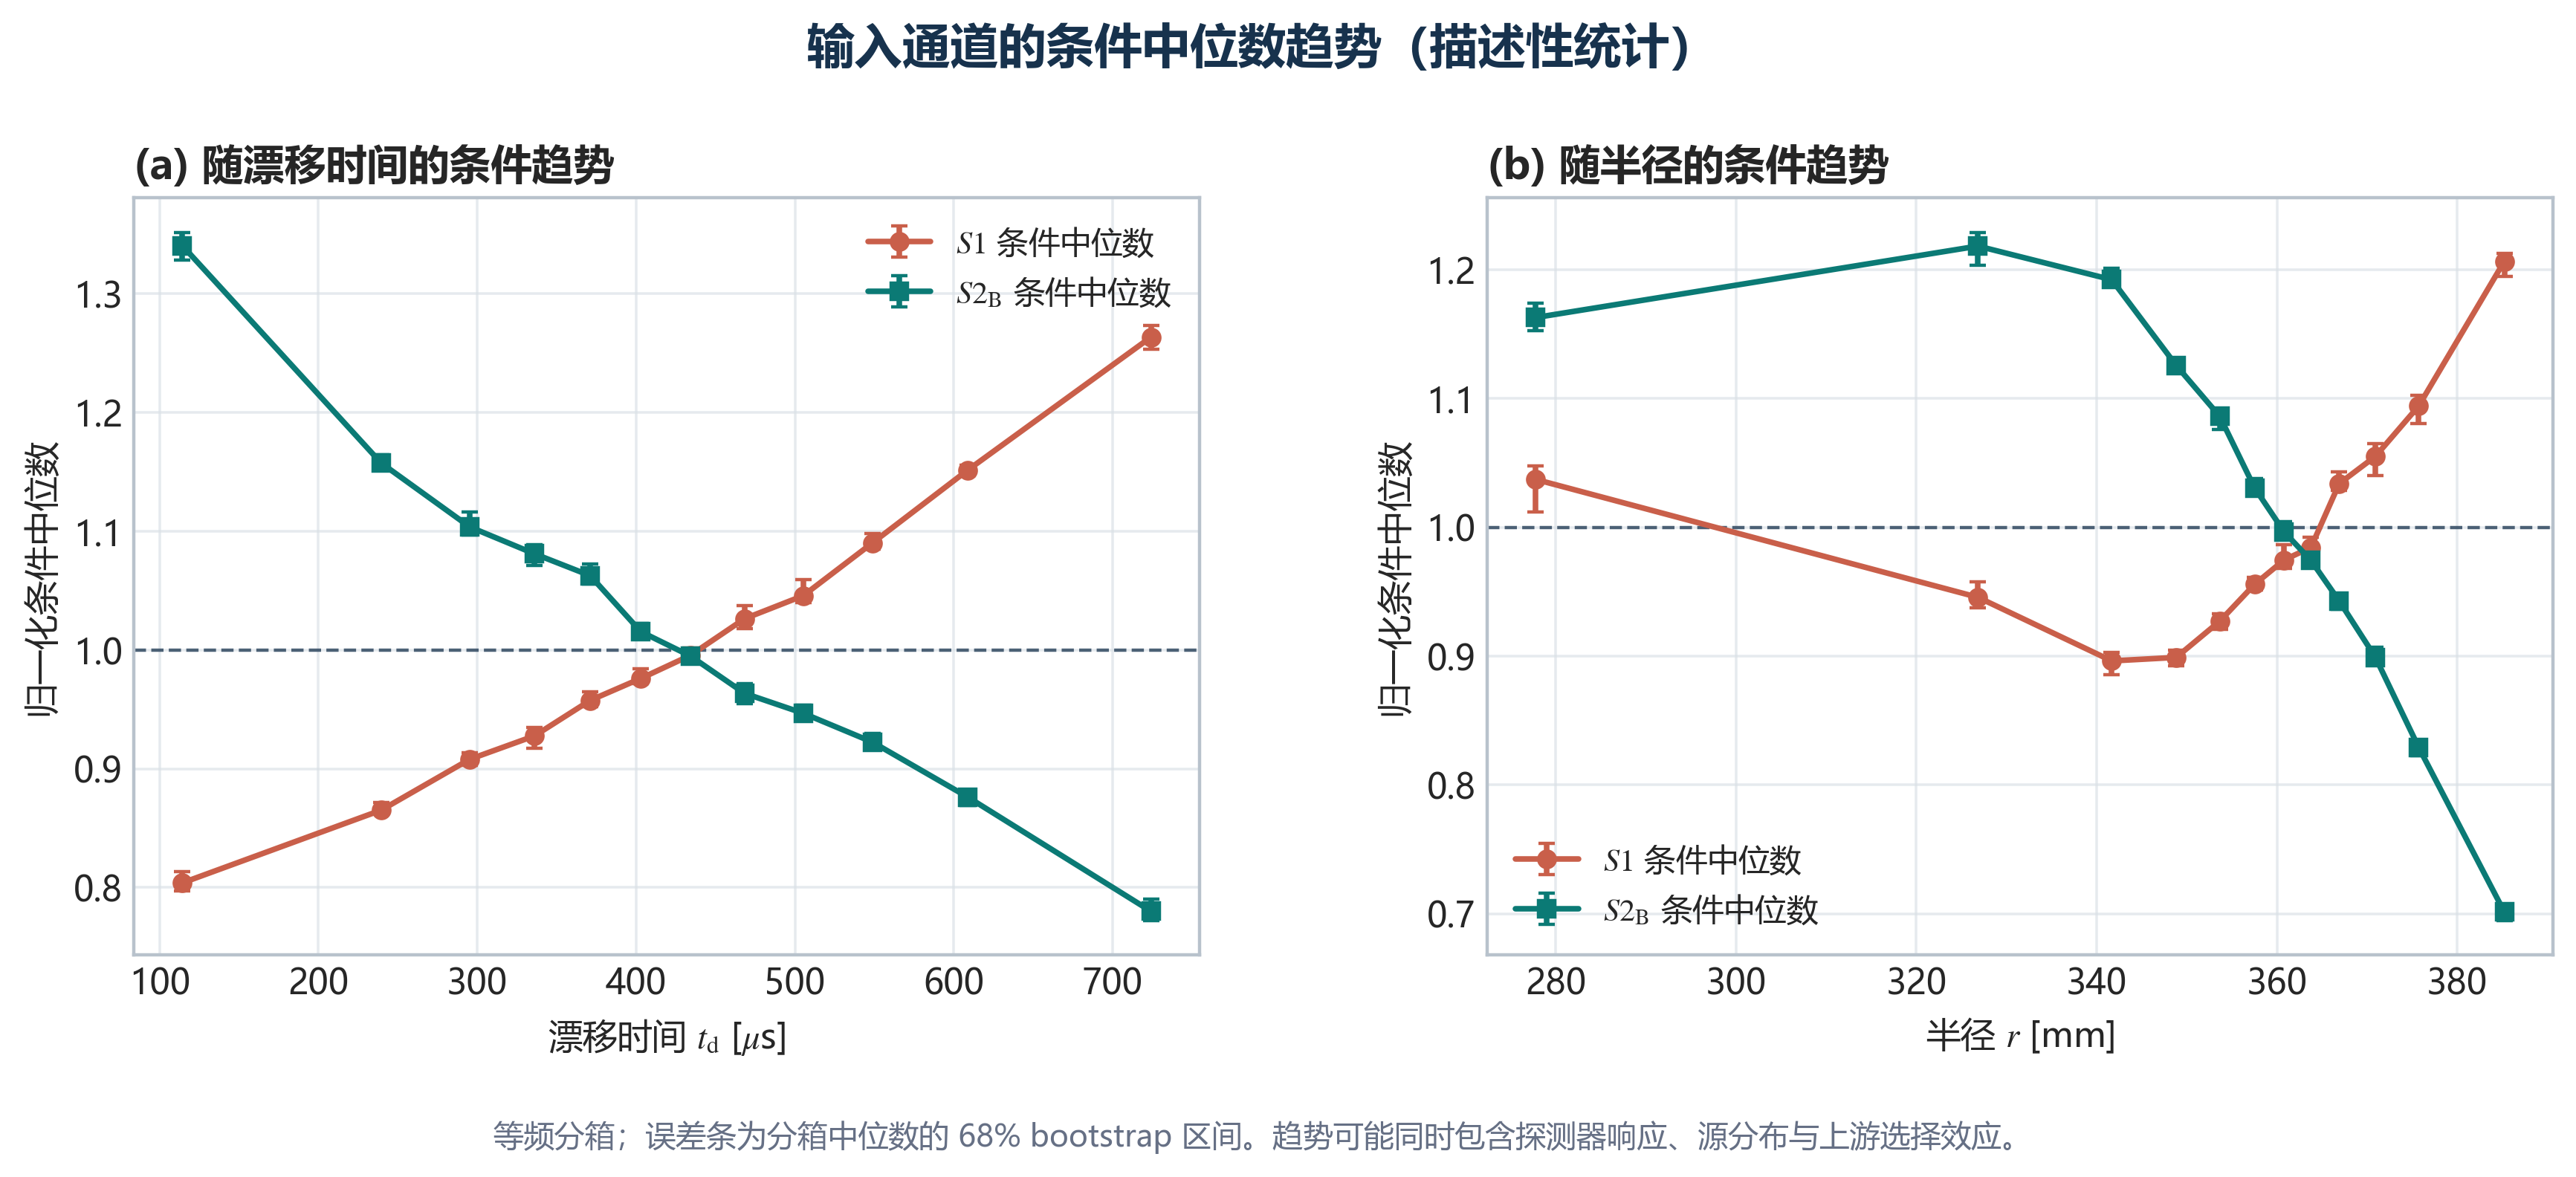
\includegraphics[width=0.94\textwidth]{04_conditional_trends_cn.png}
  \caption{S1 与 S2B 条件中位数随漂移时间和半径的变化。点为等频分箱中位数；误差条为以事件行为重采样单元的 68\% bootstrap 区间。}
\end{figure}

两条信号通道随漂移时间和半径呈现不同方向、不同幅度的变化，说明只修正单个通道可能破坏原有的 S1--S2B 补偿关系。因此后续分析需要保留“单通道修正”和“双通道联合修正”的完整消融比较。

\begin{infobox}[title={本报告确认的五件事},fonttitle=\bfseries]
\begin{enumerate}
  \item 当前输入是 4500 行、188 列的筛选后标量表；
  \item 项目只把 S1、S2B、漂移时间和两个横向坐标作为物理观测量；
  \item \texttt{sourceRow} 只负责一一对齐，不是物理特征；
  \item S1 与 S2B 具有清楚的反相关和位置结构；
  \item 样本空间覆盖明显不均匀，正式结论仍需独立 run 与更完整元数据。
\end{enumerate}
\end{infobox}

\begin{scopebox}
本报告没有进行能量校正，也没有把分布宽度称为最终能量分辨率。下一册《数据处理方法报告》说明怎样以事件级 OOF 方式学习并评价修正；第三册《数据结果分析报告》给出数值结果。
\end{scopebox}

\begin{conclusionbox}
原始数据已经提供了进行独立能量重建所需的基础信号和位置信息，但它是单一 run 的非均匀、预筛选样本；结果必须在这一边界内解释。
\end{conclusionbox}
\clearpage

\end{document}
